\begin{frame}
	\frametitle{Freeciv}

	\begin{columns}
		
		\column{0.6\textwidth}
		\begin{itemize}
			\item<1-> Versión \textcolor{UDCpink}{\textit{open source}} y \textcolor{UDCpink}{gratuita} de Sid Meier's Civilization creado en la universidad de Aarhus.
			
			\vspace{1em}
			
			\item<2-> Juego de \textcolor{UDCpink}{estrategia por turnos}.
			
			\vspace{1em}
			
			\item<3-> El jugador controla a un \textcolor{UDCpink}{grupo de colonos}, comienza en el año \textcolor{UDCpink}{4000 A.C}.
			
			\vspace{1em}
			
			\item<4-> El objetivo final es crear una \textcolor{UDCpink}{gran civilización}. Para ello existen \textcolor{UDCpink}{5 formas} de finalizar el juego:
			
			\vspace{0.5em}
			
			\begin{itemize}
				\item Victoria por \textcolor{UDCpink}{dominación}, \textcolor{UDCpink}{científica}, \textcolor{UDCpink}{religión}, \textcolor{UDCpink}{cultural} o \textcolor{UDCpink}{por puntuación}.
			\end{itemize}
		\end{itemize}

		\column{0.4\textwidth}
		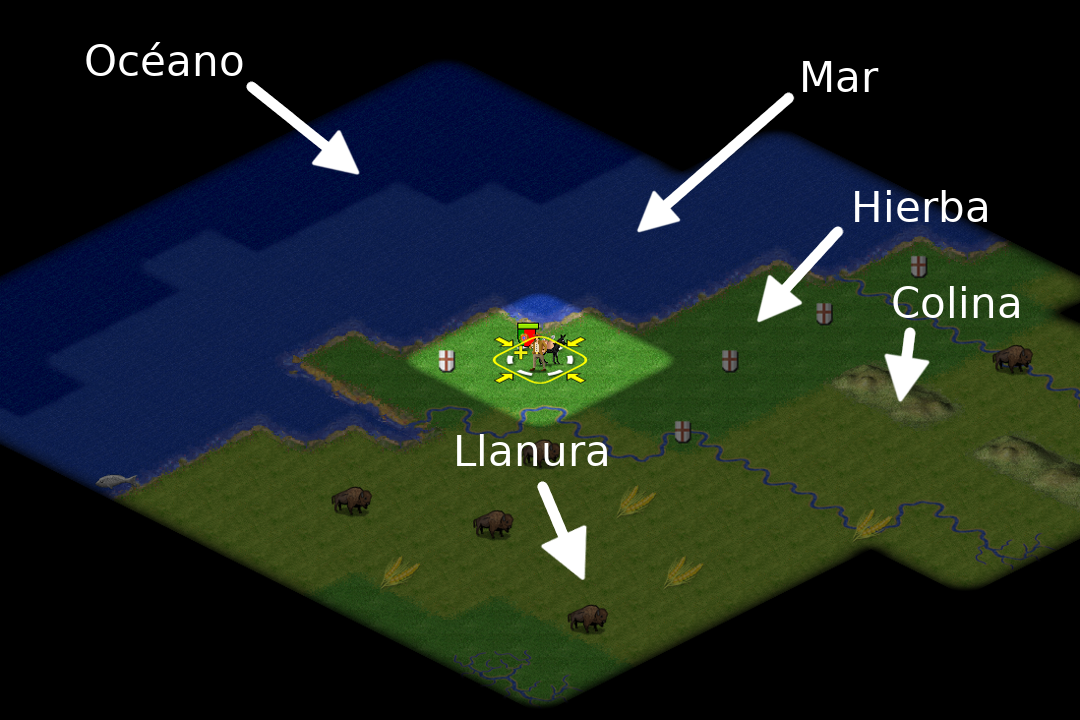
\includegraphics[width=\textwidth]{images/freeciv-example.png}
	\end{columns}

\end{frame}

\begin{frame}
\frametitle{Tipos de terrenos en Freeciv}

\begin{itemize}
	\item Hay \textcolor{UDCpink}{12 tipos de terreno}, con posibles bonificaciones.
\end{itemize}

\vspace{0.5em}

\centering
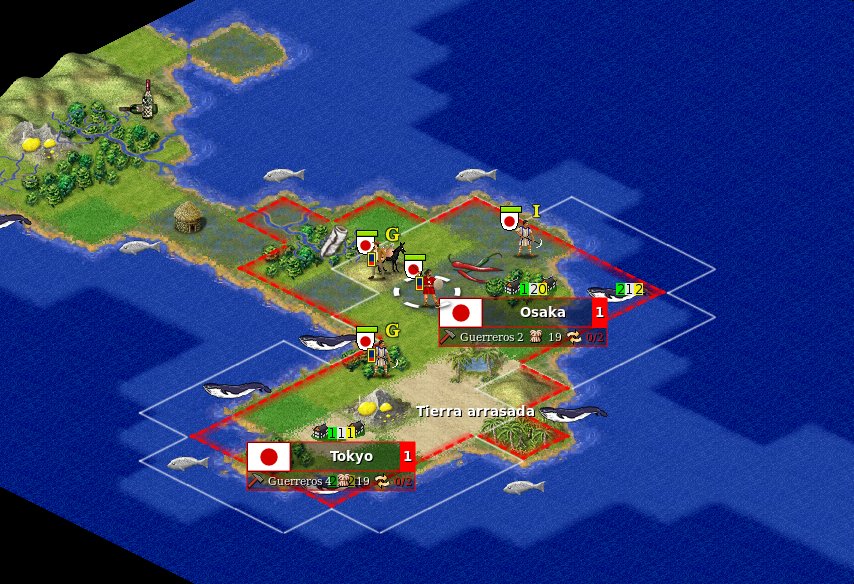
\includegraphics[width=0.8\textwidth]{images/ejemplo-partida.png}
\end{frame}


\begin{frame}
\frametitle{Objetivos del proyecto}

Para este proyecto:

\vspace{1em}

\begin{itemize}
	\item<1-> Se definirá un \textcolor{UDCpink}{modelo declarativo} del escenario para Freeciv usando \textcolor{UDCpink}{\itshape Answer Set Programming}.
	
	\vspace{1em}
	
	\item<2-> Se construirá una pequeña \textcolor{UDCpink}{herramienta gráfica} con la que manipular el escenario.
	
	\vspace{1em}
	
	\item<3-> Eficiencia: reducir o podar el número de combinaciones posibles.
\end{itemize}

\end{frame}
